\documentclass[letter,11pt]{article}
\usepackage[pdftex]{graphicx}
\usepackage{float}
\usepackage{amsmath}
\begin{document}
	\begin{center}
		\Large\textbf{CSCI 567-Machine Learning Assignment-3}
	\end{center}
	
	\section{Kernel Methods}
	
	\section{Support Vector Machines}


	\begin{equation}
		 \min_{R,\textbf{c},\varepsilon}\frac{1}{2}R^2 + C\sum_{n}\varepsilon_n \\
	\end{equation}
	\begin{equation}
		s.t. ||\phi(x_i) - b||_2^2 \leq R^2 + \varepsilon_n \\
	\end{equation}
	\begin{equation}
		\varepsilon_n \geq 0
	\end{equation}
	
	We take the Lagrangian of this primal.
	\begin{equation}
	 \mathcal{L}(R,b,\varepsilon,\alpha,\eta) = \frac{1}{2}R^2 + C \sum_{n} \varepsilon_n + \sum_{n} \alpha_n[(\phi(x_n)-b)'(\phi(x_n)-b)-R^2-\varepsilon_n] - \sum_{n}\eta_n\varepsilon_n 
	\end{equation}
	
	Let's take derivatives of primal variables and equal to 0.
	
	\begin{equation}
	\frac{\partial \mathcal{L}}{\partial R} = R - 2R \sum_{n} \alpha_n = 0 \rightarrow \sum_{n} \alpha_n = \frac{1}{2}
	\end{equation}
	
	Using this equation,
	\begin{equation}
	\frac{\partial \mathcal{L}}{\partial b} = 2 \sum_{n} \alpha_n b - 2 \sum_{n} \alpha_n \phi(x_n) = 0 \rightarrow b = 2\sum_{n} \alpha_n \phi(x_n)
	\end{equation}
	\begin{equation}
	\frac{\partial \mathcal{L}}{\partial \varepsilon} = C - \alpha_n - \eta_n = 0 \rightarrow \alpha_n + \eta_n = C
	\end{equation}
	
	If we fill this equations in Lagrangian
	\begin{equation}
		\begin{aligned}
	 \mathcal{L}(R,b,\varepsilon,\alpha,\eta) = \frac{1}{2}R^2 +  C\sum_{n}\varepsilon_n + \sum_{n} \alpha_n k(x_n,x_n) - 2\sum_{n}\alpha_n \phi(x_n)^Tb + b^Tb\sum_{n}\alpha_n - \\ R^2 \sum_{n} \alpha_n - \sum_{n}(\alpha_n + \eta_n)\epsilon_n
		\end{aligned}
	\end{equation}
		
	Using new constraints, we simplify this equation.
	
	\begin{equation}
	\mathcal{L}(R,b,\varepsilon,\alpha,\eta) = \sum_{n} \alpha_n k(x_n,x_n) - \frac{1}{2}b^Tb
	\end{equation}
		
	Dual of this LP is
	
	\begin{equation}
		\max_\alpha \sum_{n} \alpha_n k(x_n,x_n) - 2 \sum_{i}\sum_{j}\alpha_i \alpha_j k(x_i,x_j)
	\end{equation}
	$\sum_{n} \alpha_n = \frac{1}{2}$ and $k(x_n,x_n)$ is a constant. So, our LP is
	
	\begin{equation}
	\arg\min_\alpha 2 \sum_{i}\sum_{j}\alpha_i \alpha_j k(x_i,x_j)
	\end{equation}
	\begin{equation}
	0 \leq \alpha_n \leq C, \forall 
	\end{equation}
	\begin{equation}
	\sum \alpha_n = \frac{1}{2}
	\end{equation}
	
	$\alpha_n$ must be less or equal than $C$ since $\alpha_n + \eta_n = C$ and $\eta_n \geq 0$\\
	
	
	Let's find R value. $\alpha_n = C$ for abnormal values. And, for any data point that is on the boundary $ 0 \leq \alpha_n \leq C$. Also, we can say that $||\phi(x_n) - b||_2^2 = R^2$ for data points on the boundary.
	\begin{equation}
	||\phi(x_n) - b||_2^2 = R^2
	\end{equation}
	\begin{equation}
	b = 2\sum \alpha_n \phi(x_n)
	\end{equation}
	\begin{equation}
	R^2 = k(x_i,x_i) - 2 \sum_{j} \alpha_j k(x_i,x_j) + \sum_{i} \sum_{j} \alpha_i\alpha_j k(x_i,x_j)
	\end{equation}
	
	\section{Boosting}
	
	\section{Bias-Variance Trade-off}
	\subsection{Closed Form Solution and Distribution of $\hat{\beta_\lambda}$}
	
	\begin{equation}
	\hat{\beta_\lambda} = \arg \min_{\hat{\beta_\lambda}} \bigg\{\frac{1}{n}\sum_{i=1}^{n}(y_i-x_i^T\beta)^2 + \lambda||\beta||_2^2\bigg\}
	\end{equation}
	
	Define $Y$ $nx1$ matrix for $n$ data point. $X$ $pxn$ matrix for $n$ data points in $p-1$-dimension. In this case.
	
	\begin{equation}
	\hat{\beta_\lambda} = \arg \min_{\hat{\beta_\lambda}} \bigg\{(Y-X^T\beta)'(Y-X^T\beta) +\beta\lambda I\beta \bigg\}
	\end{equation}
	$$ = (Y^T-\beta^TX)(Y-X^T\beta) + \beta^T\lambda I \beta$$
	$$ = Y^TY - Y^TX^T\beta-\beta^TXY + \beta^TXX^T\beta + \beta^T\lambda I \beta$$
	\begin{equation}
	\frac{\partial \hat{\beta_\lambda}}{\partial \beta} = XY - XY + 2XX^T\beta + 2\lambda I \beta = 0
	\end{equation}	
	\begin{equation}
	\hat{\beta_\lambda} = (XX^T + \lambda I)^{-1} XY
	\end{equation}















		\section{Multinomial Logistic Regression}
		
		\section{Programming Questions}
		\begin{center}
			\begin{tabular}{|c| c |c |c|} 
				\hline
				Method & Data Type & Training Acc & Test Acc \\ [0.5ex] 
				\hline
				Batch Gradient & raw & 0.8692 & 0.8817 \\ 
				\hline
				Batch Gradient & standardized & 0.9300 & 0.9261 \\
				\hline
				Newton's Method & raw & 0.8935 & 0.8922 \\
				\hline
				Newton's Method & standardized & 0.8935 & 0.8922 \\
				\hline
				glmfit & raw & 0.9357 & 0.9265 \\
				\hline
			    glmfit & standardized & 0.9357 & 0.9265 \\
				\hline
			\end{tabular}
		\end{center}
%	\begin{figure}[H]%                 use [hb] only if necceccary!
%	\centering
%	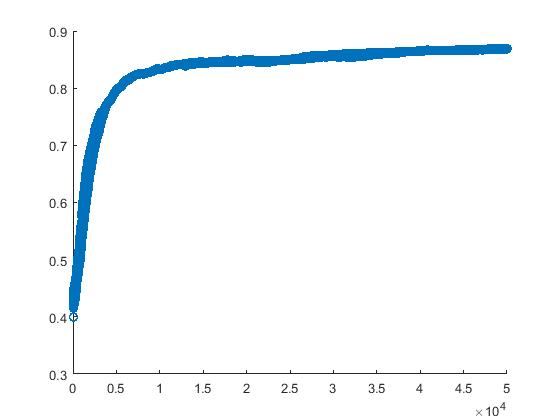
\includegraphics[width=9cm]{C:/Users/okazk_000/Desktop/Spring 2016/CSCI 567/HW2/hw2/accTrainGrad.jpg}
%	\caption{Batch Gradient over 50.000 iterations}
%	\label{fig:test}
%	\end{figure}
	\subsubsection{Chosen 20 Features}
	The feature IDs chosen according to Mutual Information values:\\
	$[52,53,56,21,55,7,16,57,25,19,24,5,27,17,3,26,23,6,11,2]$
	
	Using these 20 features on glmfit function: 
	Training accuracy = $0.8914$ and Testing Accuracy = $0.8926$
	
	\subsection{Generative Model and Discriminative Model}
	\subsubsection{MLE Parameters When Variances Are Independent}
	
	Component Proportions = ([0.2941,0.2679,0.4379])\\
	$\mu$ Parameters = ([1.538,0.0354; -1.593,1.596; -1.486,-1.408])\\
	$\Sigma$ Parameters  =\\
	First Component \hspace{15mm} Second Component \hspace{15mm} Third Component
	0.9988    0.0102 \hspace{25mm}  1.0197   -0.4525 \hspace{25mm}      1.0280    0.5110
    0.0102    3.9734  \hspace{25mm} -0.4525    1.0105 \hspace{24mm}      0.5110    1.1234\\
    Testing Accuracy = 0.9007
    
    \subsubsection{MLE Parameters When Variances Are Equal}
	Component Proportions = ([0.293,0.275,0.430])\\
	$\mu$ Parameters = ([1.549,0.0435;-1.759,-0.739;-1.385,0.0282])\\
	$\Sigma$ Parameters  =\\
	0.977 -0.004\\
	 -0.004 3.331\\
	Testing Accuracy = 0.7600
	
	\subsubsection{Multinomial Logistic Model}
	Testing Accuracy = 0.8846
	
	\subsubsection{Plot and Analysis}	
		 
		 We can see that the the best decision boundaries are given by Gaussian Mixture Model with different variance. And the worst one is given by Gaussian Mixture Model with same variance.\\
		 
		 
		 It is obvious that variances of three Gaussian models are different from each other. Even though green and blue colored data points have a similar variance, red colored data points' distribution has much larger variance. Since we made the same variance assumption in second model, it is reasonable to get not a very good decision boundary.\\
		 
		 On the other hand, logistic regression has made a very good classification and draw a good decision boundary between classes even though it couldn't use the advantage of being nonlinear as different variance Gaussian Mixture Model did.
		 
		 
		 
	 \subsubsection{Subset Training Data}
	 3 plots below shows the testing accuracy w.r.t. training data sizes for three models.


	\subsection{Practical Logistic Regression on Toy Data}
	\subsubsection{Discretization}
	The best model is chosen according to the best cross-validation accuracy. Leave one out technique is used.
		\begin{center}
			\begin{tabular}{|c| c |c |c | c |} 
				\hline
				Data & Best Discretization & Training Acc & Test Acc & Heldout Acc\\ [0.5ex] 
				\hline
				1 & $16^2$ & 0.9950 & 0.9737 & 0.9775 \\ 
				\hline
				2 & $16^2$ & 0.9975 & 0.9949 & 0.9925 \\
				\hline
				3 & $16^2$ & 1 & 0.9950 & 1 \\
				\hline
				4 & $4^2$ & 0.9800 & 0.9539 & 0.9675\\
				\hline
			\end{tabular}
		\end{center}	 
	\subsubsection{$\l$2 norm regularization)}
	For Data1:		
		\begin{center}
			\begin{tabular}{|c| c |c |c | c |} 
				\hline
				Type & $\lambda = 1$ &  $\lambda = 0.1$  &  $\lambda = 0.01$  &  $\lambda = 0.001$ \\ [0.5ex] 
				\hline
				Training Accuracy & 0.9700 & 0.9750 & 0.9775 & 0.9775 \\ 
				\hline
				Heldout Accuracy & 0.9700 & 0.9700 & 0.9700 & 0.9700 \\
				\hline
				Testing Accuracy & 0.9559 & 0.9583 & 0.9611 & 0.9612 \\
				\hline
			\end{tabular}
		\end{center}
	For Data2:		
	\begin{center}
		\begin{tabular}{|c| c |c |c | c |} 
			\hline
			Type & $\lambda = 1$ &  $\lambda = 0.1$  &  $\lambda = 0.01$  &  $\lambda = 0.001$ \\ [0.5ex] 
			\hline
			Training Accuracy & 0.9850 & 0.9850 & 0.9825 & 0.9825 \\ 
			\hline
			Heldout Accuracy & 0.9825 & 0.9825 & 0.9800 & 0.9800 \\
			\hline
			Testing Accuracy & 0.9833 & 0.9871 & 0.9915 & 0.9915 \\
			\hline
		\end{tabular}
	\end{center}
	For Data3:		
	\begin{center}
		\begin{tabular}{|c| c |c |c | c |} 
			\hline
			Type & $\lambda = 1$ &  $\lambda = 0.1$  &  $\lambda = 0.01$  &  $\lambda = 0.001$ \\ [0.5ex] 
			\hline
			Training Accuracy & 0.9800 & 0.9850 & 0.9900 & 0.9950 \\ 
			\hline
			Heldout Accuracy & 0.9800 & 0.9800 & 0.9800 & 0.9800 \\
			\hline
			Testing Accuracy & 0.9741 & 0.9760 & 0.9779 & 0.9783 \\
			\hline
		\end{tabular}
	\end{center}
	For Data4:		
	\begin{center}
		\begin{tabular}{|c| c |c |c | c |} 
			\hline
			Type & $\lambda = 1$ &  $\lambda = 0.1$  &  $\lambda = 0.01$  &  $\lambda = 0.001$ \\ [0.5ex] 
			\hline
			Training Accuracy & 0.9525 & 0.9800 & 0.9800 & 0.9825 \\ 
			\hline
			Heldout Accuracy & 0.9425 & 0.9675 & 0.9550 & 0.9625 \\
			\hline
			Testing Accuracy & 0.9425 & 0.9539 & 0.9520 & 0.9587 \\
			\hline
		\end{tabular}
	\end{center}
	\subsubsection{Visualization}
		For regularized terms; for Data2  $\lambda$ chosen as 1 and for Data3 $\lambda$ is chosen as 0.1.//
		For unregularized models for data2 and data3 are both $16^2$ discretizations.
		
		 
								
\end{document}